\documentclass{article}
\usepackage{tikz}
\usepackage{caption}

\begin{document}

\begin{figure}[h!]
    \centering
    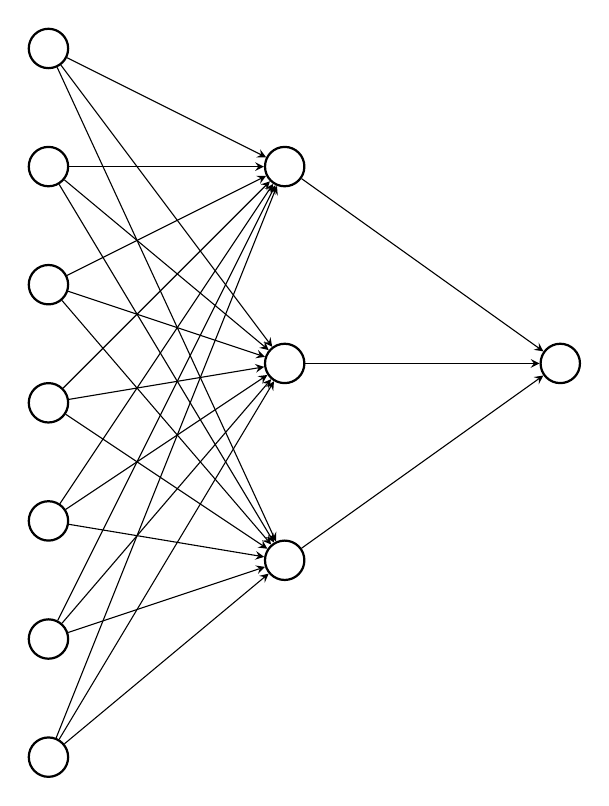
\begin{tikzpicture}[
        neuron/.style={circle, thick, draw=black, minimum size=0.5cm},
        layer/.style={draw=none},
        ->, >=stealth
    ]

    % Input layer (5 neurons)
    \foreach \i in {1,...,7}
        \node[neuron] (I\i) at (0, -\i*1.5) {};

    % Hidden layer (3 neurons)
    \foreach \i in {1,...,3}
        \node[neuron] (H\i) at (3, -\i*2.5-0.5) {};

    % Output layer (1 neuron)
    \node[neuron] (O1) at (6.5, -5.5) {};

    % Connections: Input to Hidden
    \foreach \i in {1,...,7}
        \foreach \j in {1,...,3}
            \draw (I\i) -- (H\j);

    % Connections: Hidden to Output
    \foreach \i in {1,...,3}
        \draw (H\i) -- (O1);

    \end{tikzpicture}
\end{figure}

\end{document}
